\chapter{Entwurfsmuster}
\label{ch:Entwurfsmuster}

In diesem Kapitel soll exemplarisch die Verwendung von klassischen Entwurfsmustern gezeigt und begründet werden.
Außerdem wird die Verwendung der Entwurfsmuster jeweils mit einem UML-Klassendiagramm verdeutlicht.
\newline
Allgemein sind Entwurfsmuster wiederverwendbare und generalisierte Lösungen für häufige Problemstellungen.
Durch die Generalisierung müssen Entwurfsmuster teilweise für konkrete Anwendungsfälle angepasst werden, sodass die endgültige Lösung vom eigentlichen Entwurfsmuster abweichen kann.
Deshalb werden in den folgenden Abschnitten insbesondere auch die Abweichungen vom Muster in Reinform dokumentiert. 

\section{Composite}

\begin{figure}[h]
    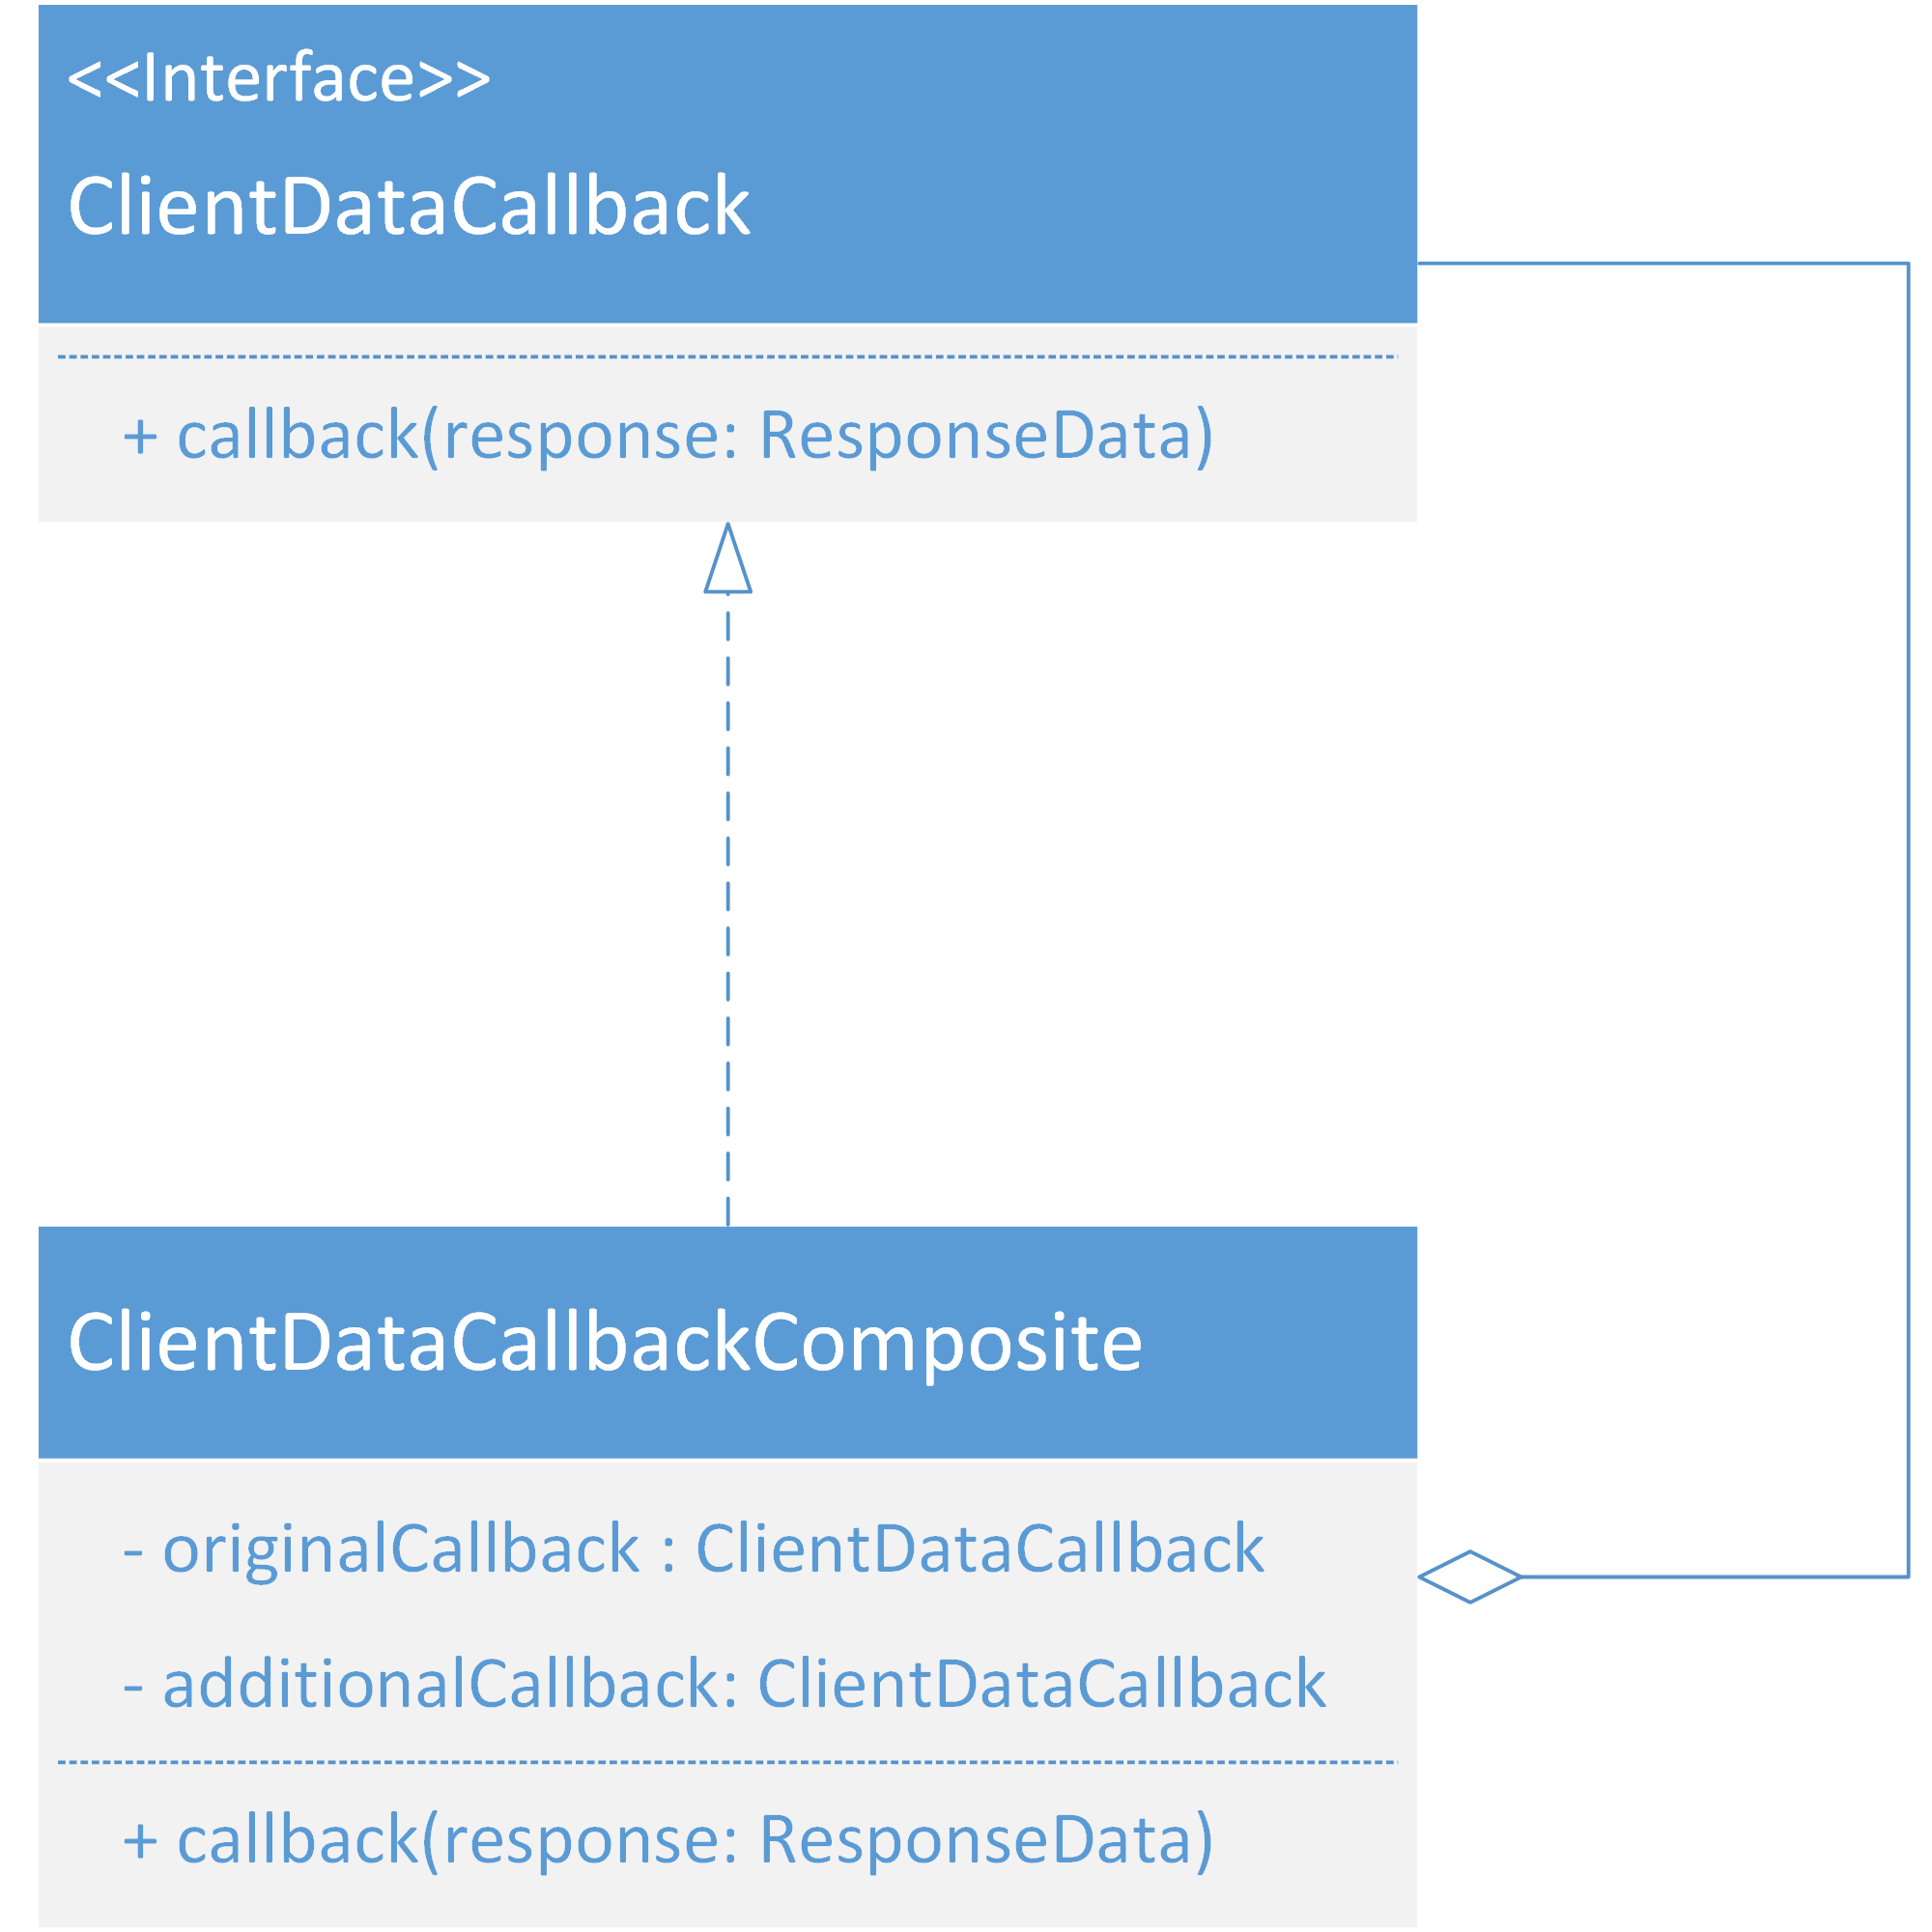
\includegraphics[scale=0.4]{pattern_composite.png}
    \centering
    \caption{Umsetzung des Composite Patterns}
    \label{fig:pattern_composite}
\end{figure}

\newpage
\section{Strategy}

\begin{figure}[h]
    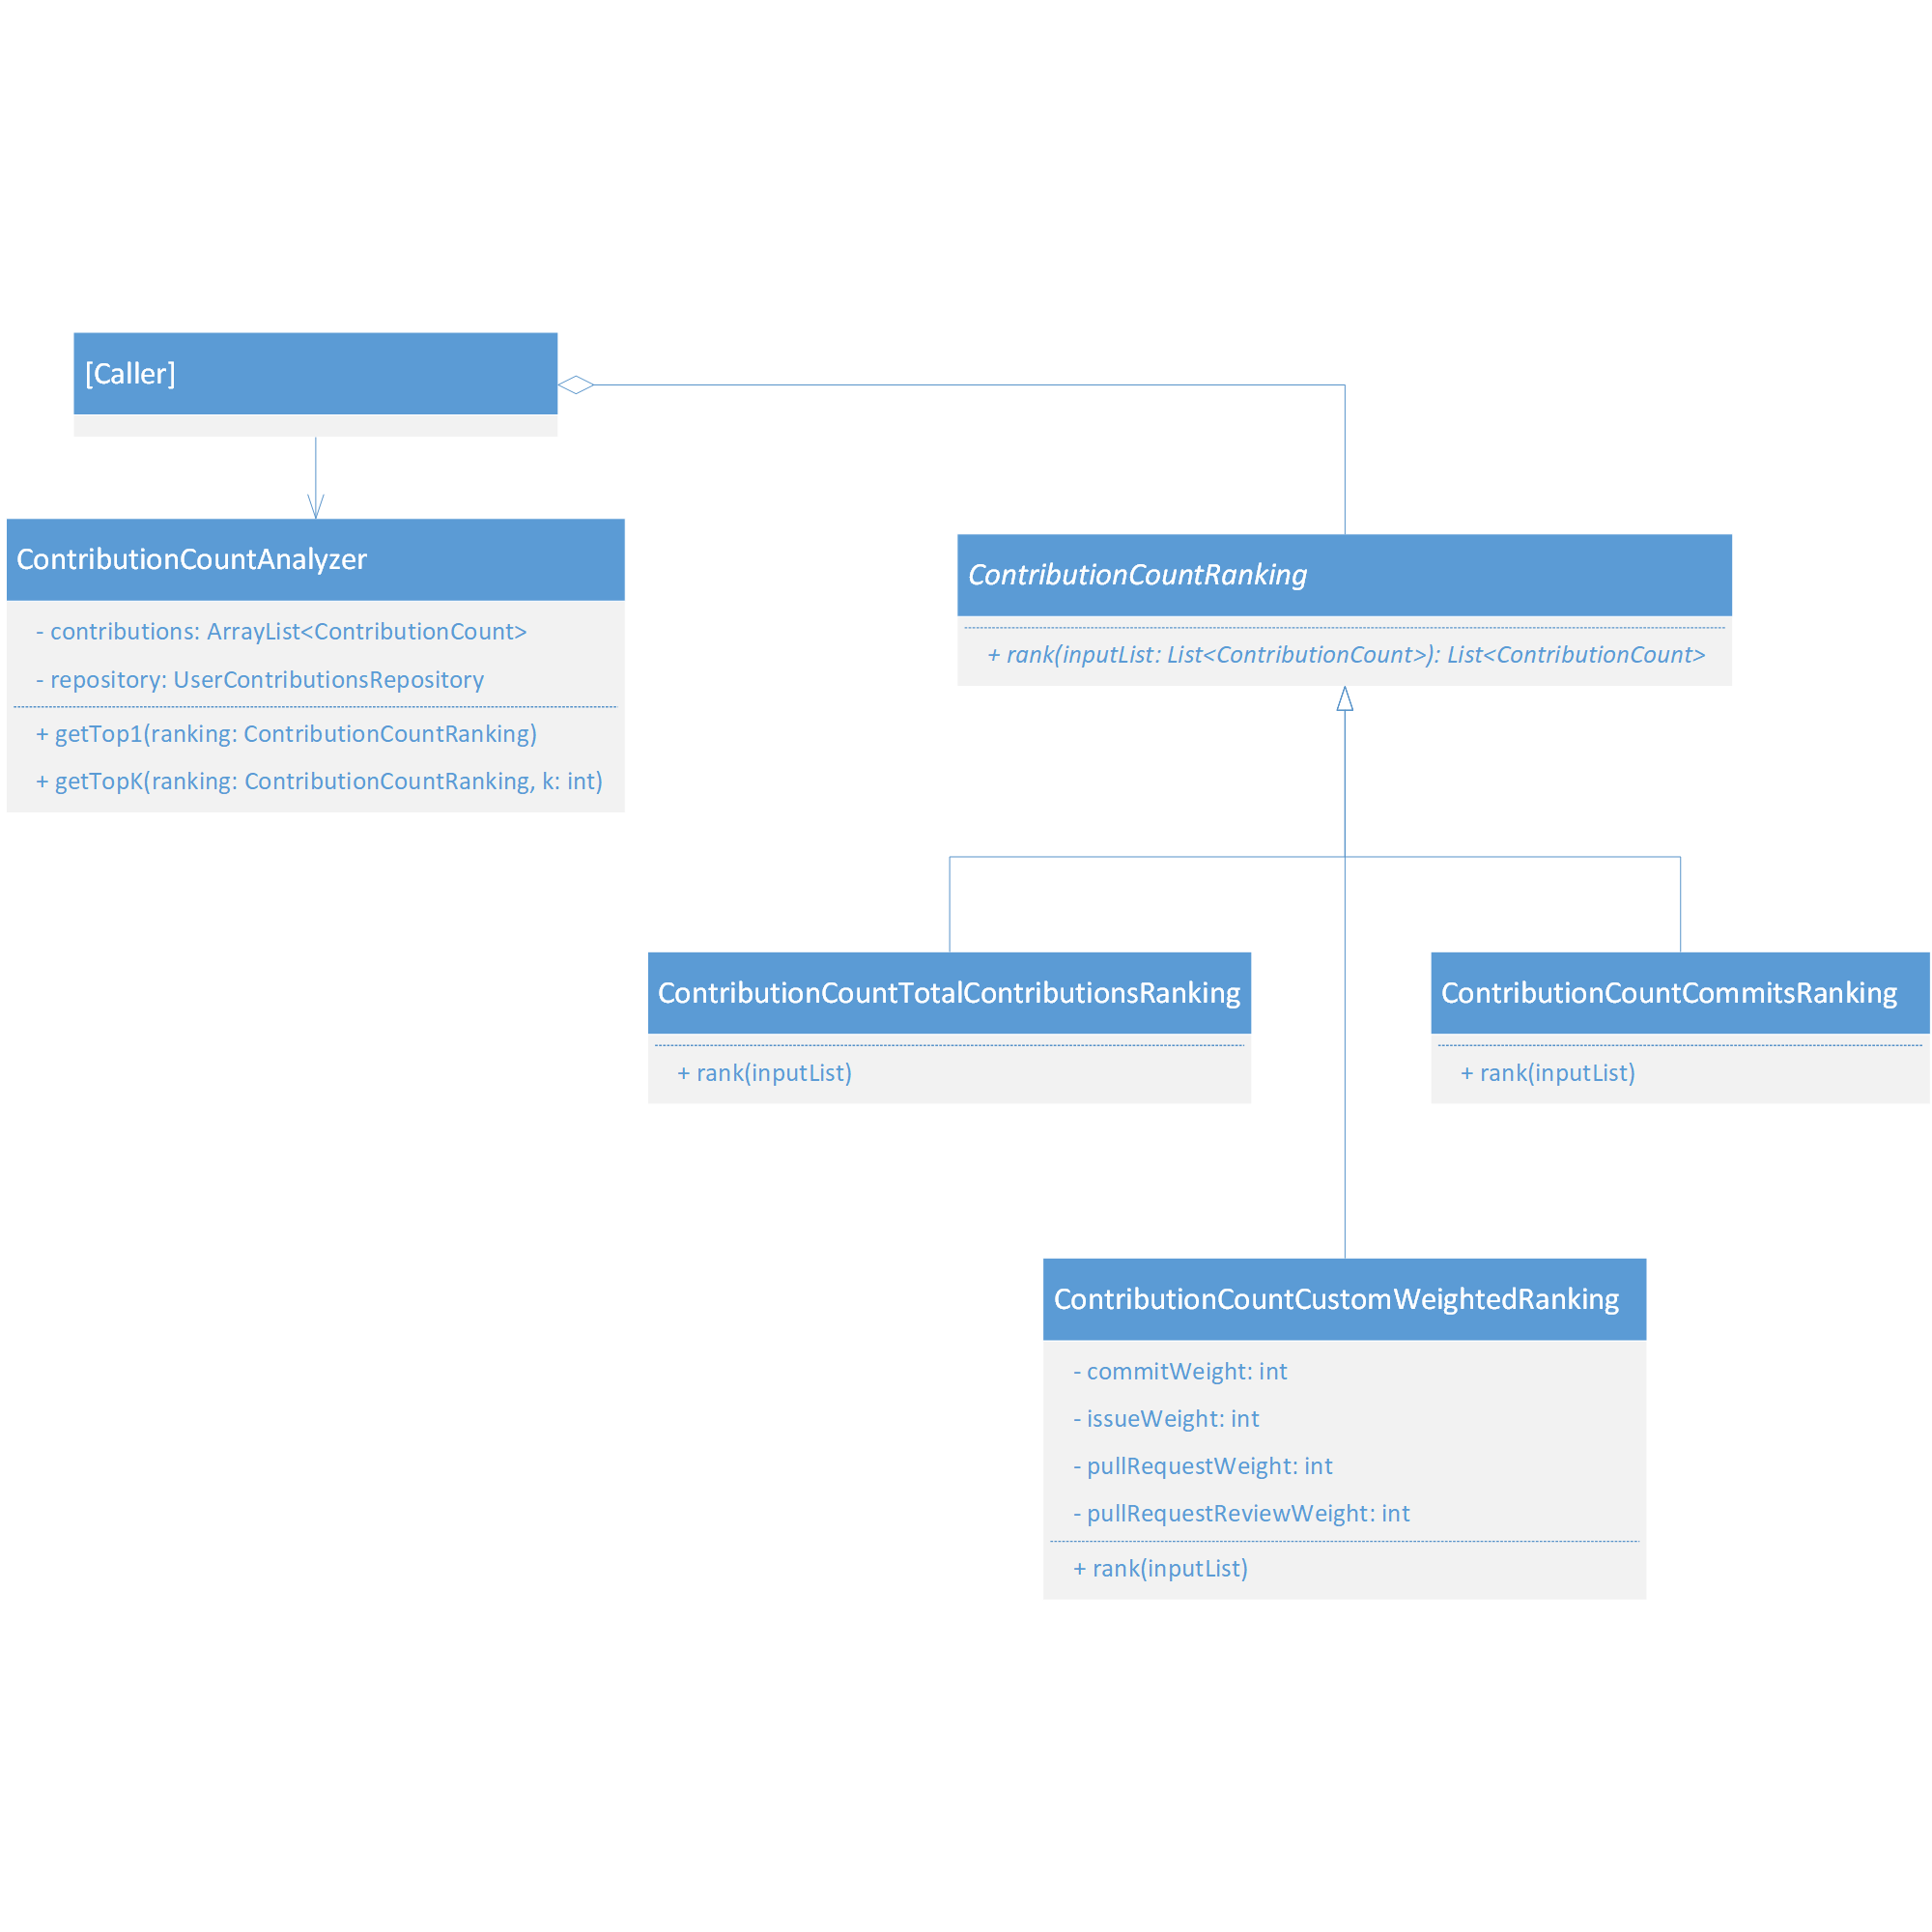
\includegraphics{pattern_strategy.png}
    \centering
    \caption{Umsetzung des Strategy-Patterns}
    \label{fig:pattern_strategy}
\end{figure}

